\documentclass[11pt,a4paper]{article}
\pdfoutput=1

\usepackage{jcappub}
\usepackage[T1]{fontenc}
\usepackage{lmodern}
\usepackage{microtype}
\usepackage{bm}
\usepackage{booktabs}

\newcommand{\PR}{\mathcal P_{\mathcal R}}
\newcommand{\Mpc}{\mathrm{Mpc}}
\newcommand{\dd}{\mathrm d}
\newcommand{\trans}{\mathsf T}
\hypersetup{
  pdftitle={Reconstructing the primordial power spectrum with FrediPy: a proof of concept},
  pdfauthor={Kay Lehnert},
  pdfkeywords={Bayesian reasoning, CMBR theory, cosmological perturbation theory}
}

\title{Reconstructing the primordial power spectrum with FrediPy: a proof of concept}
\author{Kay Lehnert}
\affiliation{National University of Ireland, Maynooth}
\emailAdd{k.lehnert@protonmail.com}

\abstract{
The CMB temperature spectrum is a linear integral transform of the primordial
curvature spectrum when the background cosmology and transfer functions are
fixed.  This makes it a natural test case for FrediPy, a general Python package
for Bayesian inversion of Fredholm integral equations.  We formulate the CMB
projection as a Gaussian-process inverse problem and retain only the ingredients
needed for a transparent proof of concept.  First, we reconstruct a known power
law from synthetic, unlensed CLASS temperature data.  On the fixed range
$3\times10^{-4}<k<0.15\,\Mpc^{-1}$, the posterior mean differs from the input by
at most $7.5\times10^{-4}$ fractionally.  We then apply the same public FrediPy
interface to Planck PR3 high-$\ell$ TT bandpowers, keeping the cosmology,
lensing template and calibration fixed while varying the Gaussian-process
hyperparameters in a small sensitivity scan.  At the reference values and on
the range with direct noise-weighted operator sensitivity, the flexible
posterior mean differs from its best-fitting power law by at most $1.24\%$ and
$0.48$ pointwise posterior standard deviations.  Their data quadratics are
$218.5$ and $218.9$, respectively.  Factor-two changes of either RBF
hyperparameter keep the maximum separation below $2.9\%$.  FrediPy therefore
passes the controlled reconstruction test, while the observational example
gives no reason to replace a featureless power law in this conditional setting.
The latter is an illustration, not a feature-significance or
cosmological-parameter analysis.
}

\keywords{Bayesian reasoning, CMBR theory, cosmological perturbation theory}
\compress
\notoc

\begin{document}
\maketitle
\flushbottom

\section{Introduction}
\label{sec:introduction}

A power law provides the standard two-parameter description of primordial
fluctuations,
\begin{equation}
  \PR(k)=A_s\left(\frac{k}{k_*}\right)^{n_s-1} .
  \label{eq:power-law}
\end{equation}
It is nearly scale invariant and becomes a straight line when both axes are
logarithmic.  CMB observations are consistent with this form
\citep{planck2018vi,planck2018x}, but they do not measure $\PR(k)$ directly.
They measure angular spectra after acoustic
evolution and projection along the line of sight.  Reconstructing the input
from the output is therefore an inverse problem.

There is a long history of approaching this problem through deconvolution,
regularised direct inversion, knots and other non-parametric descriptions
\citep{shafieloo2004,gauthier2012,hunt2014,sohn2022,raffaelli2025,chaki2025}.
The common difficulty is physical rather than algorithmic: many primordial
functions project to almost the same angular spectrum.  A reconstruction must
state which combinations of $\PR$ the data constrain and how the remaining
freedom is regularised.

FrediPy was developed as a general solver for this class of problem
\citep{fredipy,horak2022}.  It places a Gaussian-process prior on an unknown
function and conditions that process on noisy linear integral constraints.
Although its initial applications concerned spectral functions, neither its
mathematics nor its software interface is tied to that setting.  The primordial
spectrum is a particularly clean cosmological example because the unlensed CMB
spectra are Fredholm integrals of the first kind at fixed cosmology.

Our contribution is deliberately narrow: we do not introduce another
primordial-spectrum reconstruction algorithm.  Instead, we supply the
CMB-specific operator, data vector and covariance to the unmodified public
FrediPy interface.  This provides an inspectable test of whether a general
Fredholm solver developed for QCD spectral functions can both recover a CLASS
input and condition on Planck bandpowers.

Here we ask whether FrediPy can recover a known primordial spectrum from CLASS
and whether the same construction can be
shown on real CMB bandpowers without building a full cosmological inference
pipeline around it.  The answer to the first question is quantitative: the
input power law is recovered to better than one part in a thousand over the
tested range.  For the second, a conditional Planck TT reconstruction remains
close to an optimised power law.  This does not test inflationary models or
establish the absence of features.  It shows what the Fredholm formulation does
and where a larger analysis would have to begin.

\section{The CMB projection as a Fredholm problem}
\label{sec:fredholm}

\subsection{Forward map}

We use the dimensionless curvature spectrum defined by
\begin{equation}
 \left\langle \mathcal R(\bm k)\mathcal R(\bm k')\right\rangle
 = (2\pi)^3\delta^{(3)}(\bm k+\bm k')\,
   \frac{2\pi^2}{k^3}\PR(k).
 \label{eq:pr-definition}
\end{equation}
For fixed late-time parameters and unlensed scalar perturbations, the
temperature spectrum is
\begin{equation}
 C_\ell^{TT}=4\pi\int \dd\ln k\,
 \PR(k)\left|\Delta_\ell^T(k)\right|^2 ,
 \label{eq:cmb-fredholm}
\end{equation}
where $\Delta_\ell^T$ is the temperature transfer function.  CLASS computes
the transfer functions and the corresponding angular spectra
\citep{blas2011}.  Equation~\eqref{eq:cmb-fredholm} has the standard Fredholm
form
\begin{equation}
 g(x)=\int \dd t\,G(x,t)f(t).
 \label{eq:fredholm-generic}
\end{equation}
Here $x$ labels a multipole or bandpower, $t=\ln k$, the unknown is $f=\PR$,
and the kernel contains the squared radiation transfer function.

The kernel is broad and oscillatory.  Projection mixes neighbouring
wavenumbers, while Silk damping and the finite observed multipole range remove
information.  Inverting equation~\eqref{eq:cmb-fredholm} without
regularisation would amplify small numerical or observational fluctuations.
Figure~\ref{fig:operator} visualises the discretised response.  It also makes
clear why a CMB experiment constrains a range of $k$, rather than each node
independently.

\begin{figure}[htb]
  \centering
  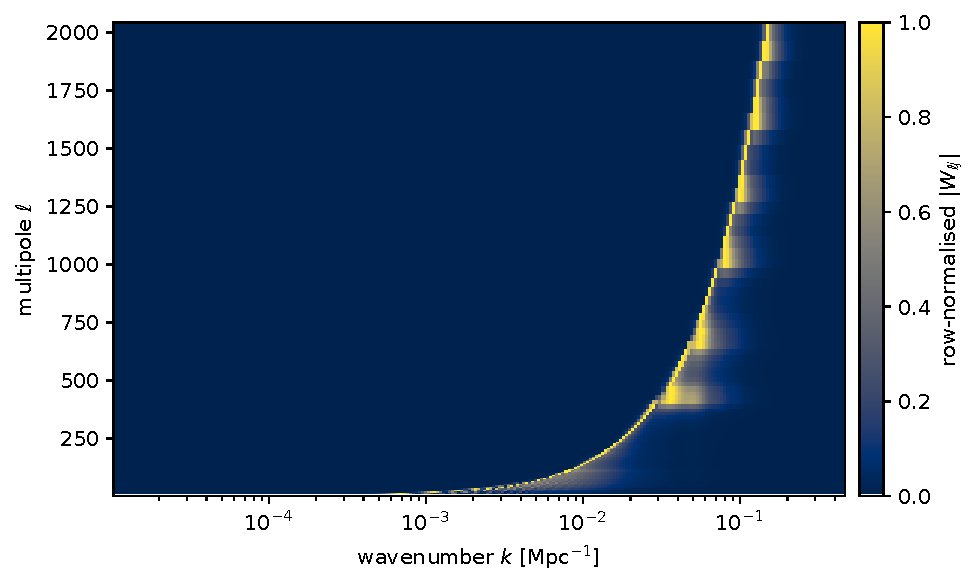
\includegraphics[width=0.92\linewidth]{figures/fredholm_operator.pdf}
  \caption{The discretised synthetic CLASS operator.  Each row maps the
  primordial spectrum on the $\ln k$ grid to one temperature datum; rows are
  normalised for visibility.  The broad response and its changing support are
  the source of the inverse problem.}
  \label{fig:operator}
\end{figure}

For the numerical calculation we set $u=\ln k$ and work with the order-unity
field
\begin{equation}
 f(u)=\frac{\PR(e^u)}{A_0},\qquad A_0=2.1\times10^{-9}.
\end{equation}
Quadrature and, for Planck, the bandpower windows turn the forward map into
\begin{equation}
 \bm y=\bm W\bm f+\bm\epsilon,
 \qquad \bm\epsilon\sim\mathcal N(\bm 0,\bm\Sigma).
 \label{eq:discrete-forward}
\end{equation}
The matrix $\bm W$ includes $A_0$ and therefore predicts the data in their
physical units.  We keep the dimensionless spectrum and the $\dd\ln k$ measure
explicit throughout.

\subsection{Gaussian-process inversion}

We assign $f$ a Gaussian-process prior with mean $m$ and radial-basis-function
kernel
\begin{equation}
 K(u,u')=\sigma_f^2
 \exp\left[-\frac{(u-u')^2}{2\gamma^2}\right].
 \label{eq:rbf}
\end{equation}
Our reference choice in both calculations is $m=1$, $\sigma_f=1$ and
$\gamma=1.5$.  The mean is a scale-invariant spectrum, not the tilted power
law that we later reconstruct.  The prior permits smooth departures over
order-unity intervals in $\ln k$.  We keep $m=1$ fixed and vary the two RBF
hyperparameters in table~\ref{tab:gp-sensitivity}.  A feature analysis should
instead infer or marginalise over them.

Because equations~\eqref{eq:discrete-forward} and \eqref{eq:rbf} are Gaussian
and linear, the posterior is analytic \citep{rasmussen2006,valentine2020}:
\begin{align}
 \overline{\bm f}
 &=\bm m+\bm K\bm W^\trans
   (\bm W\bm K\bm W^\trans+\bm\Sigma)^{-1}
   (\bm y-\bm W\bm m),
 \label{eq:posterior-mean}\\
 \bm K_{\rm post}
 &=\bm K-\bm K\bm W^\trans
   (\bm W\bm K\bm W^\trans+\bm\Sigma)^{-1}
   \bm W\bm K.
 \label{eq:posterior-covariance}
\end{align}
The posterior returns to the prior where $\bm W$ has little sensitivity.  That
behaviour is part of the answer: an apparently smooth extrapolation outside the
supported range must not be mistaken for a measurement.

FrediPy provides the Gaussian process, covariance kernel, integral operator and
linear noisy constraint that evaluate these expressions.  Our adapter passes
the precomputed cosmological quadrature to its public \texttt{Integral} and
\texttt{LinearEquality} classes.  Since the FrediPy process is zero-mean, the
adapter conditions on $\bm y-\bm W\bm m$ and adds $\bm m$ back afterwards.  It
passes \texttt{cov\_y}$=\bm\Sigma$ as a covariance---not a vector of standard
deviations.  The repository tests the returned mean and covariance against a
separate dense Gaussian evaluation of
equations~\eqref{eq:posterior-mean}--\eqref{eq:posterior-covariance}.

\section{Controlled reconstruction from CLASS}
\label{sec:synthetic}

The first test should answer one question without observational complications:
if the input spectrum is known, does the full chain recover it?  We generate an
unlensed scalar TT spectrum with CLASS~3.3.4 using
\begin{equation}
 A_s=2.1\times10^{-9},\qquad n_s=0.9649,
 \qquad k_*=0.05\,\Mpc^{-1}.
\end{equation}
We use flat scalar adiabatic initial conditions and fix
$h=0.6736$, $\omega_b=0.02237$, $\omega_{\rm cdm}=0.1200$,
$\tau_{\rm reio}=0.0544$, $N_{\rm ncdm}=0$ and $N_{\rm ur}=3.044$.  The
density parameters are Planck-like \citep{planck2018vi}, but the absence of a
massive-neutrino species is part of this proof-of-concept setup.  We sample 125
multipoles between $\ell=2$ and 2000 and reconstruct on 240 logarithmic nodes
covering $1.05\times10^{-5}<k<0.455\,\Mpc^{-1}$.

For this synthetic test we convert \texttt{CLASS.raw\_cl} to the conventional
rescaled spectrum
\begin{equation}
 D_\ell\equiv\frac{\ell(\ell+1)}{2\pi}C_\ell .
 \label{eq:dell}
\end{equation}
The deterministic $D_\ell$ values form the target vector; no random noise
realisation is added.  We assign a diagonal covariance with standard
deviations $\sigma_\ell=0.01D_\ell$, or variances $(0.01D_\ell)^2$, to define a
simple conditioning problem.  This covariance is a numerical convention for
this closure test, not a model of cosmic variance or an experiment.  The operator
is constructed independently from the CLASS line-of-sight sources and a finer
$k$ quadrature.  Its direct forward spectrum agrees with
\texttt{CLASS.raw\_cl} to a maximum fractional difference of
$9.42\times10^{-4}$ across the sampled multipoles.

\begin{figure}[htb]
  \centering
  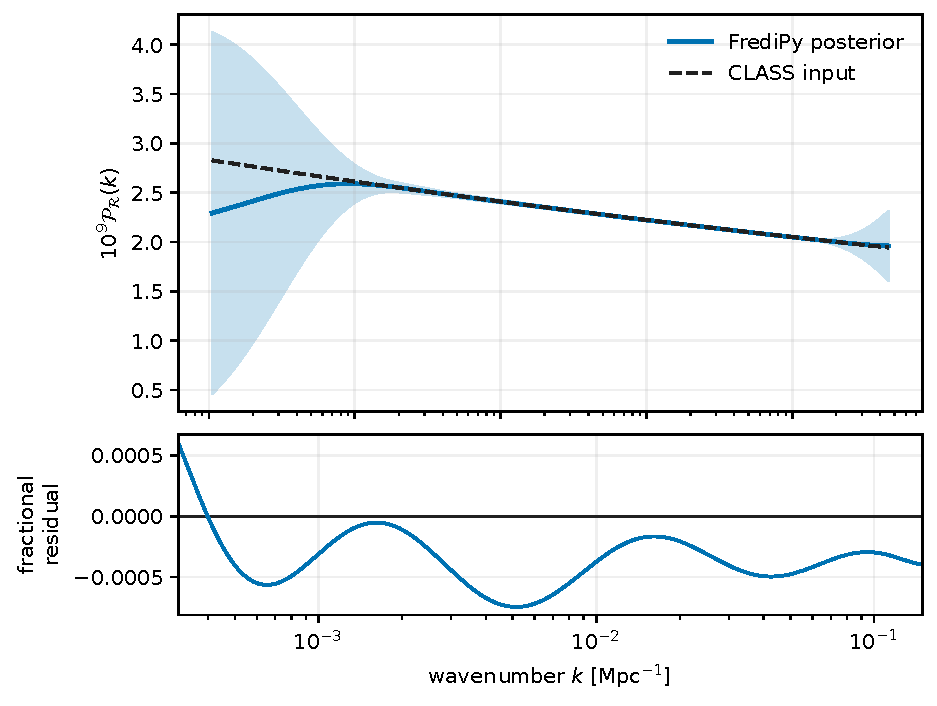
\includegraphics[width=0.94\linewidth]{figures/synthetic_reconstruction.pdf}
  \caption{Controlled CLASS reconstruction.  The upper panel compares the
  injected primordial power law with the FrediPy posterior mean and its
  $\pm1$ pointwise posterior standard deviation; this is not a simultaneous
  band.  The lower panel shows the fractional reconstruction residual on the
  fixed evaluation interval.  Outside this interval, visible in the
  upper panel, the result eventually reverts towards its constant prior mean.}
  \label{fig:synthetic}
\end{figure}

Figure~\ref{fig:synthetic} shows the result.  On the fixed interval
\begin{equation}
 3\times10^{-4}<k<0.15\,\Mpc^{-1},
 \label{eq:synthetic-range}
\end{equation}
the maximum absolute fractional error of the posterior mean is
$7.46\times10^{-4}$ and the root-mean-square error is
$4.16\times10^{-4}$.  A constant spectrum at the prior mean differs from the
truth by as much as $16.3\%$ on the same interval, so the agreement is not a
trivial restatement of the prior.  Across the complete $k$ grid, by contrast,
the maximum error rises to about $19\%$ as the reconstruction loses support and
returns to $m=1$.  Quoting the restricted range is therefore essential.

This is a closure test, not an independent test of CLASS.  The target and the
transfer sources come from the same Boltzmann code, although the direct angular
spectrum and the reconstructed operator use separate numerical paths.  What it
does establish is the desired proof of concept: with the correct
dimensionless-spectrum normalisation and sufficient quadrature resolution,
FrediPy recovers the primordial power law that generated the synthetic CMB.

\section{A conditional reconstruction from Planck TT}
\label{sec:planck}

We next replace the synthetic vector by the first 215 TT bandpowers of the
Planck PR3 \texttt{plik\_lite} high-$\ell$ likelihood, covering
$30\leq\ell\leq2508$ \citep{planck2018v,planckpr3data}.  We retain the full
$215\times215$ bandpower covariance.  The exact published binning windows were
applied upstream and are encoded in the compact bandpower operator $\bm W$.
The background parameters remain fixed to the values used in the synthetic test.
The forward model consists of the unlensed linear response of
equation~\eqref{eq:cmb-fredholm} plus a fiducial lensed-minus-unlensed
bandpower template.  Calibration is fixed to unity.  Thus the dependence on
$\PR$ remains linear, at the cost of holding the lensing correction fixed.

Table~\ref{tab:setups} summarises what changes between the two calculations.
The same grid, prior and public FrediPy conditioning are used in both.

\begin{table}[htb]
\centering
\caption{The two calculations retained in the streamlined analysis.}
\label{tab:setups}
\small
\begin{tabular}{lll}
\toprule
 & Synthetic closure & Planck illustration \\
\midrule
Temperature data & CLASS-derived $D_\ell$, 125 values & PR3 high-$\ell$ TT, 215 bins \\
Covariance & diagonal, $\sigma_\ell=0.01D_\ell$ & full \texttt{plik\_lite} covariance \\
Lensing & absent & fixed additive template \\
Calibration & not applicable & fixed to unity \\
Cosmology & fixed & fixed \\
GP hyperparameters & fixed RBF & fixed RBF; sensitivity scan \\
Purpose & recovery of known truth & conditional adequacy check \\
\bottomrule
\end{tabular}
\end{table}

To identify the range to which this discretised operator is directly
sensitive, we whiten its rows using the data covariance.  If
$\bm\Sigma=\bm L\bm L^\trans$, the noise-weighted sensitivity score of
primordial node $j$ is
\begin{equation}
 s_j=\left\|\bm L^{-1}\bm W_{:j}\right\|_2.
 \label{eq:sensitivity}
\end{equation}
We report comparisons where $s_j$ is at least 1\% of its maximum.  This selects
89 contiguous nodes over the interval, rounded to three significant figures,
\begin{equation}
 k\in[0.00399,0.204],\Mpc^{-1}.
\label{eq:planck-range}
\end{equation}
The threshold is an explicit reporting convention rather than a confidence
boundary.

For comparison with the flexible posterior, we fit the two parameters of
equation~\eqref{eq:power-law} at $k_*=0.05\,\Mpc^{-1}$ using the same operator,
lensing template and covariance.  We minimise
\begin{equation}
 Q=(\bm d-\bm t)^\trans\bm\Sigma^{-1}(\bm d-\bm t).
 \label{eq:q}
\end{equation}
Here $\bm d$ is the observed bandpower vector and $\bm t$ is the prediction.
The optimum is
\begin{equation}
 A_s=2.094\times10^{-9},\qquad n_s=0.961,
 \label{eq:planck-power-law}
\end{equation}
with $Q=218.90$.  Evaluating the FrediPy posterior mean in the same forward
model gives $Q=218.51$.  For reference, the unoptimised fiducial power law
$(A_s,n_s)=(2.1\times10^{-9},0.9649)$ gives $Q=225.37$.

\begin{figure}[htb]
  \centering
  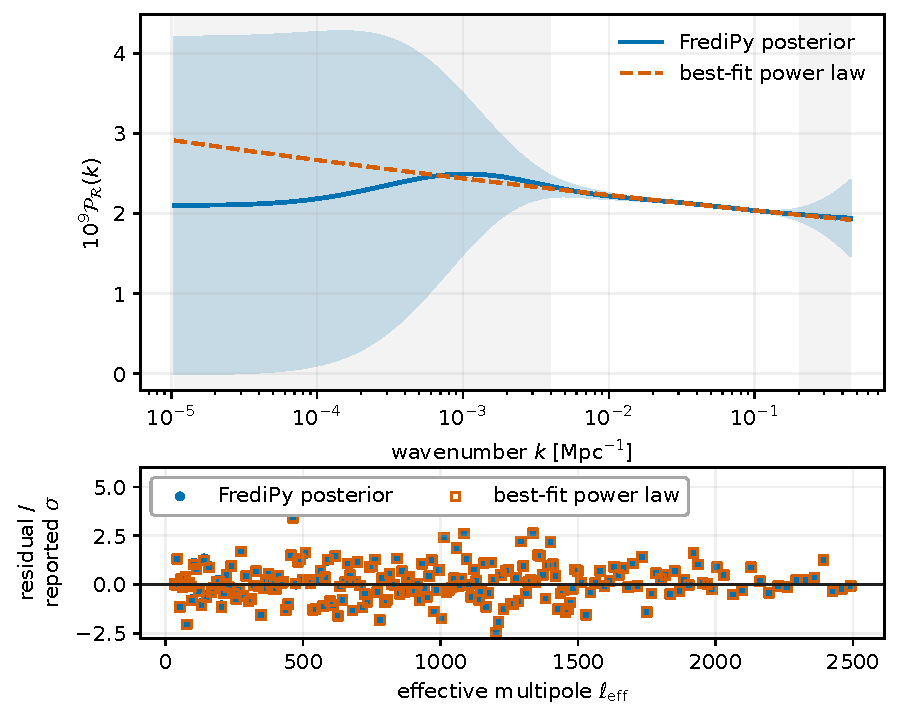
\includegraphics[width=0.94\linewidth]{figures/planck_reconstruction.pdf}
  \caption{Conditional Planck PR3 reconstruction.  The FrediPy posterior mean
  and its $\pm1$ pointwise posterior standard deviation are compared with the
  best-fitting power law of equation~\eqref{eq:planck-power-law}; the band is
  not simultaneous, and grey regions lie outside the direct-sensitivity range.
  The lower panel shows the bandpower residuals divided by the reported
  diagonal errors.  Their correlations are retained in the fits and in the
  quoted $Q$ values.}
  \label{fig:planck}
\end{figure}

Within the sensitivity range, the posterior mean and best-fitting power law
differ by at most $1.24\%$, with a root-mean-square difference of $0.334\%$.
Their largest pointwise separation is $0.48$ posterior standard deviations,
and every retained node lies within one pointwise standard deviation.  As
figure~\ref{fig:planck} shows, the non-parametric reconstruction is therefore
pointwise close to a straight line in $\ln\PR$ versus $\ln k$.  The improvement
$\Delta Q=0.39$ of the flexible posterior mean is small; moreover, $Q$ alone
does not penalise the freedom of a function.  We consequently do not interpret
it as evidence for primordial features.

Within this small scan, the qualitative Planck result is not peculiar to the
reference hyperparameters.  Halving or doubling either RBF hyperparameter
keeps the maximum separation from the fitted power law below $2.9\%$ and
$\Delta Q$ at
or below $1.80$, as table~\ref{tab:gp-sensitivity} shows.  A deliberately
shorter correlation length, $\gamma=0.5$, permits a $5.38\%$ separation and
gives $\Delta Q=3.45$.  This is the expected direction: reducing $\gamma$
admits finer structure.  The scan keeps the cosmology, lensing template,
calibration, prior mean and reporting range fixed.  It is not a substitute for
hyperparameter marginalisation or a global feature test.

\begin{table}[htb]
\centering
\caption{Hyperparameter sensitivity of the conditional Planck reconstruction.
The maximum fractional difference between the flexible posterior mean and the
same best-fitting power law is evaluated over the 89-node sensitivity range.
All other assumptions are fixed.  The difference
$\Delta Q=Q_{\rm PL}-Q_{\rm flexible}$ is descriptive; it is neither a
likelihood-ratio statistic nor a feature-significance measure.}
\label{tab:gp-sensitivity}
\small
\begin{tabular}{ccrc}
\toprule
$\sigma_f$ & $\gamma$ & Maximum difference & $\Delta Q$ \\
\midrule
1.0 & 1.50 & $1.24\%$ & 0.39 \\
0.5 & 1.50 & $0.63\%$ & 0.35 \\
2.0 & 1.50 & $1.48\%$ & 0.41 \\
1.0 & 0.75 & $2.88\%$ & 1.80 \\
1.0 & 3.00 & $0.39\%$ & 0.22 \\
1.0 & 0.50 & $5.38\%$ & 3.45 \\
\bottomrule
\end{tabular}
\end{table}

\section{Scope of the result}
\label{sec:scope}

The synthetic result is the central claim of this paper: FrediPy correctly
solves the CLASS primordial-spectrum inverse problem in a controlled setting.
The Planck calculation has a narrower role.  It shows that real bandpowers and
a full covariance can be supplied to the same machinery, and that the output
does not demand visible departures from a power law under the stated
conditions.

Several ingredients would have to change before turning the illustration into
a parameter constraint or feature search.  The background cosmology,
calibration and lensing response should be varied jointly with $\PR$; low-$\ell$
temperature and polarisation information should be included; foreground and
likelihood approximations should be treated at the level appropriate to the
experiment; and the kernel family should be varied.  The small sensitivity
scan above does not replace hyperparameter marginalisation.  Pointwise
posterior bands are correlated and do not define a global feature test.  The
Gaussian prior also does not enforce positivity, although the posterior means
shown here remain positive.

A fixed smoothness prior can suppress narrow features, while a more permissive
prior can fit fluctuations without making them significant.  Individual
wiggles in figure~\ref{fig:planck} therefore have no direct physical
interpretation.  A feature analysis would instead embed the reconstruction in
a joint likelihood and compare prior choices on simulated skies with known
coverage.

\section{Conclusions}
\label{sec:conclusions}

The primordial curvature spectrum provides a direct cosmological example of a
Fredholm equation.  At fixed cosmology, CLASS supplies the kernel, while
FrediPy supplies the Gaussian-process conditioning.  The resulting calculation
is small enough to inspect: a matrix forward model, a data covariance and the
closed-form posterior of equations~\eqref{eq:posterior-mean} and
\eqref{eq:posterior-covariance}.

The controlled test succeeds.  A tilted primordial power law is recovered from
synthetic CLASS TT data with a maximum fractional error below
$7.5\times10^{-4}$ on the fixed interval.  Applying the same interface to
Planck high-$\ell$ TT gives a posterior mean close to a fitted power law over
the range with direct operator sensitivity.  In this fixed setup, a featureless
power law explains the bandpowers about as well as the flexible posterior mean.
Changing the RBF hyperparameters alters the visible departures, as expected,
but the small scan does not turn them into a feature-significance result.

This example shows that FrediPy can perform the primordial-spectrum
reconstruction and provides a reproducible starting point for a later joint
CMB analysis.  It does not claim that the data exclude features or prefer a
particular inflationary model.

\section*{Data and code availability}

The accompanying repository contains the analysis code, focused tests, paper
source, figures and compact numerical inputs needed to reproduce every number
quoted here.  It recomputes the inversion through FrediPy from checksum-verified,
precomputed operators rather than loading a cached posterior.  Raw CLASS and
Planck operator generation remains provenance-linked to the larger validation
repository.  The software is released under the MIT licence; the Planck-derived
input retains its separate upstream terms.  FrediPy~0.2.1 and CLASS~3.3.4 are
cited explicitly \citep{fredipy,blas2011}.

\acknowledgments

The author acknowledges support from the John and Pat Hume Scholarship, the
Swiss Study Foundation and the Friedrich Naumann Foundation for Freedom.
OpenAI Codex (GPT-5), including delegated Codex agents, was used in August 2026
for repository restructuring, code development, numerical analysis and
cross-checks, and manuscript drafting and editing.  We remain responsible for
the scientific content, code and final manuscript.

\bibliographystyle{JHEP}
\bibliography{refs}

\end{document}
